\documentclass[a4paper,11pt]{scrartcl}

\usepackage[ngerman]{babel} 
\usepackage[T1]{fontenc}
\usepackage[utf8]{inputenc}
\usepackage{hyperref}

\usepackage{amsmath,amsfonts,amssymb}
\usepackage{graphicx}
\usepackage{siunitx}

\usepackage{epstopdf}

\setcounter{section}{3}


\begin{document}
\hfill Alexander Schnapp

\hfill Max Menges

\begin{center}
\underline{\Huge{Intro HPC: Blatt 3}}\\
\large{04.11.1014}\\
\end{center}


\subsection{Moores Law}
Nach \emph{Moores Law} verdoppelt sich die Prozessorleistung alle 18 Monate. Für die Rechneleistung $R$ gilt dann nach $a$ Jahren bei momentaner Leistung vom $R_{peak}$\footnote{\url{http://top500.org/lists/2014/06/}}:

\begin{align*}
R&=R_{peak}\cdot 2^{\frac{a}{1.5}} \Rightarrow a = 1.5\cdot \log_2{\frac{R}{R_{peak}}}
\end{align*}

Damit wird ein Exaflop nach \emph{Moores Law} in 6.28 Jahren erreicht.
\begin{align*}
1.5\cdot \log_2{\frac{1000}{54.9}}&=6.28
\end{align*}

Mit den Werten der TOP500 Liste jeweils aus dem November 2007 und 2011 ergibt sich:
\begin{align*}
    a&= \frac{4}{\log_2{\frac{R_{2011}}{R_{2007}}}}=0.94
\end{align*}

Also ein Vedopplung alle 11.3 Monate statt alle 18 Monate wie von Moore vorhergesagt. Damit wir auch ein Exaflop früher erreicht, und zwar in 3.9 Jahren.\\

\subsection{Amdahls Law}

\subsection{Measure Latency}

Der Quelltext liegt unter \verb+../3/3_3/pingpong.cpp+. Makefile zum Compilieren und ausführen liegt bei. \\

Es werden pro Nachrichtengröße jeweils 8 Nachrichten geschickt (mehr hat MPI irgendwie nicht erlaubt). 


\begin{figure}[!ht]
\centering
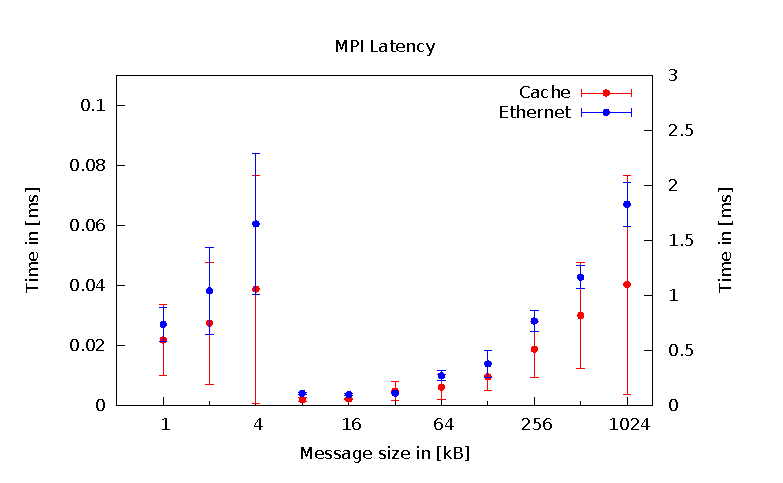
\includegraphics[width=0.7\textwidth,keepaspectratio]{3_3/data/plot.eps}
\end{figure}



\subsection{Measure Bandwidth}

\end{document}
